\documentclass{article}
%Image-related packages
\usepackage{float}
\usepackage{graphicx}
\usepackage{subcaption}
\usepackage[export]{adjustbox}
\usepackage{wrapfig}
\graphicspath{ {./images/} }
\usepackage{listings, lstautogobble}
\usepackage{listings-rust}
\usepackage[verbatim]{lstfiracode}
\usepackage{xcolor}
\usepackage{fontawesome5}
\usepackage{keystroke}
\usepackage{menukeys}
\title{How To Guide for nt-tools.exe}
\author{Ajeesh T Vijayan  \\
    MSc Cryptography  \\
    London Metropolitan University
}

\lstdefinestyle{DOS}
{
    backgroundcolor=\color{black},
    basicstyle=\scriptsize\color{white}\ttfamily
}

\date{\today}
\begin{document}

    \maketitle

    \section*{Introduction}
    This document describes how to use the command line tool developed as part of the assignments.

    \section*{How To}

    \begin{enumerate}
        \item Double clicking the ``.exe" file will open the app. Below is a screen shot of the landing page of the app.
        \begin{figure}[H]
            \centering
            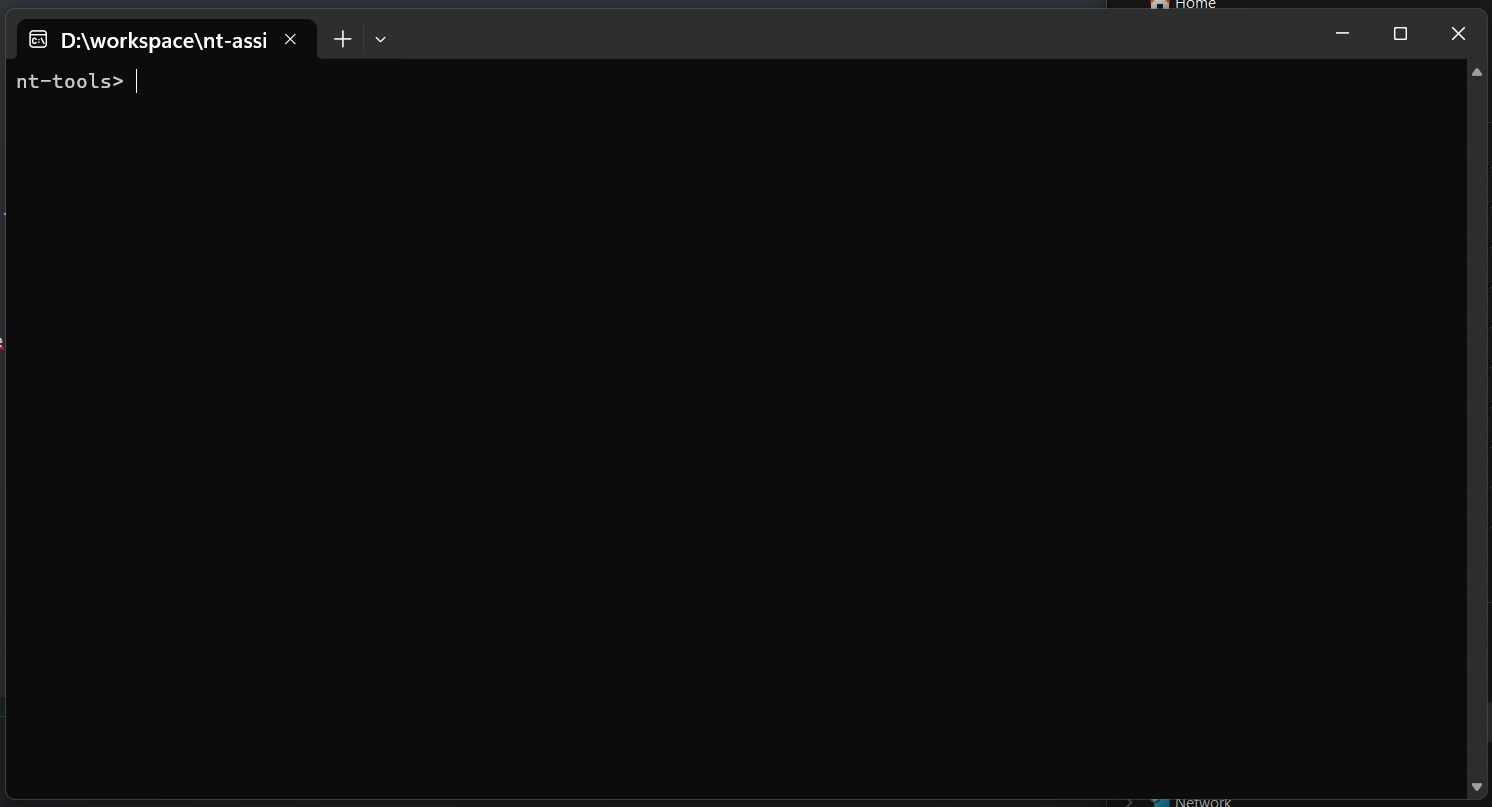
\includegraphics[scale=0.35]{landing_page.png}
            \caption{Landing Page}
        \end{figure}
        \item Typing ``help" or just pressing the ``Enter"\Return key will display the help.
        \begin{figure}[H]
            \centering
            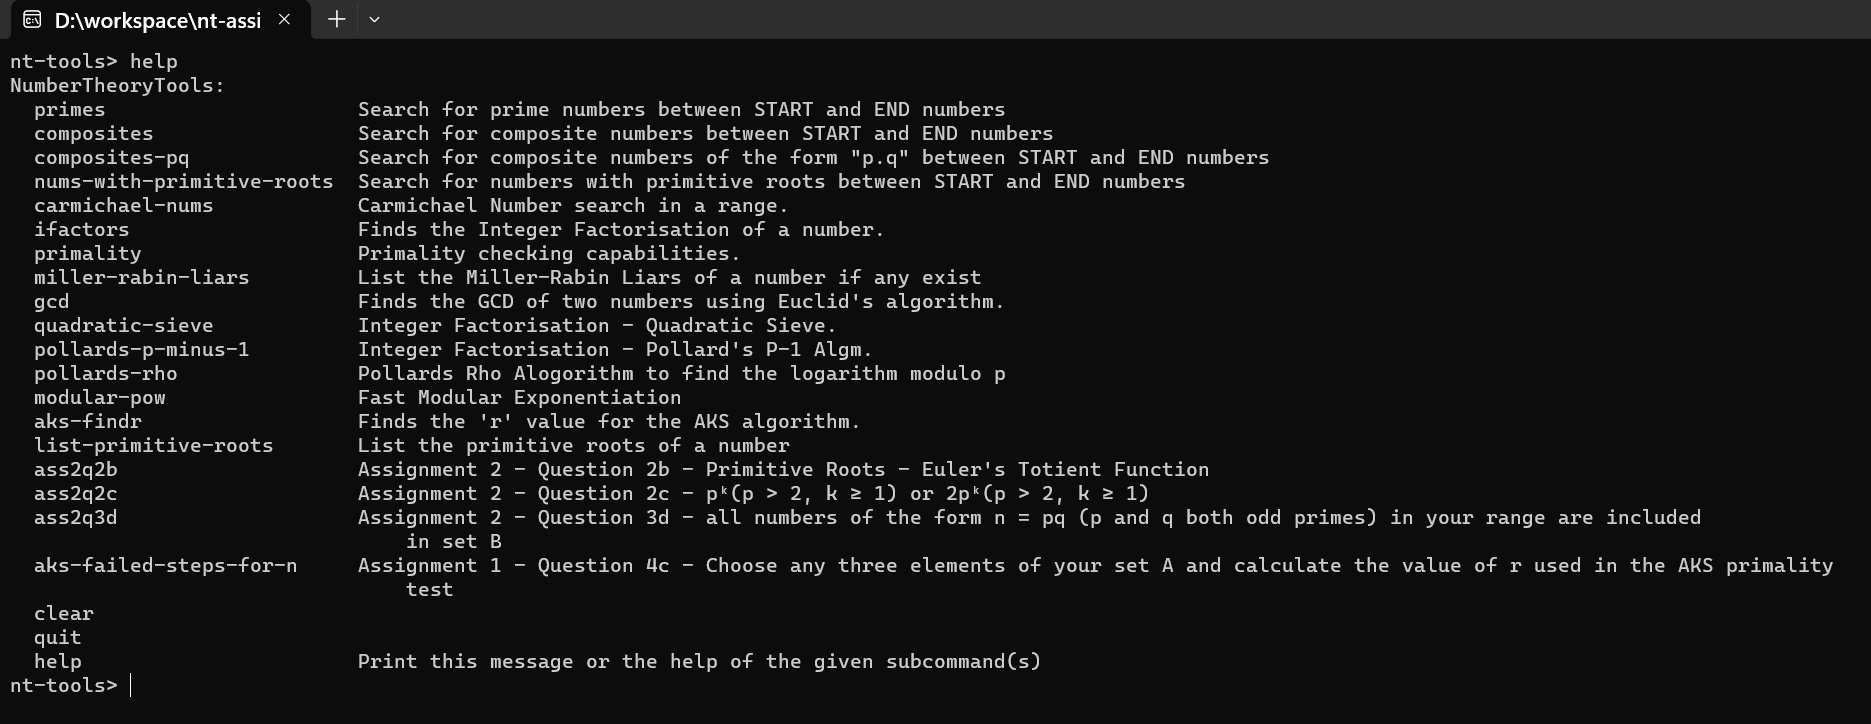
\includegraphics[scale=0.35]{help_page.png}
            \caption{Help Page}
        \end{figure}
    \end{enumerate}

    \subsection*{Command Syntax}
    \begin{enumerate}
        \item primes
        \begin{lstlisting}[style=DOS]

        primes -s 2800 -e 3100
        \end{lstlisting}

        The below screenshot shows a sample output:
        \begin{figure}[H]
            \centering
            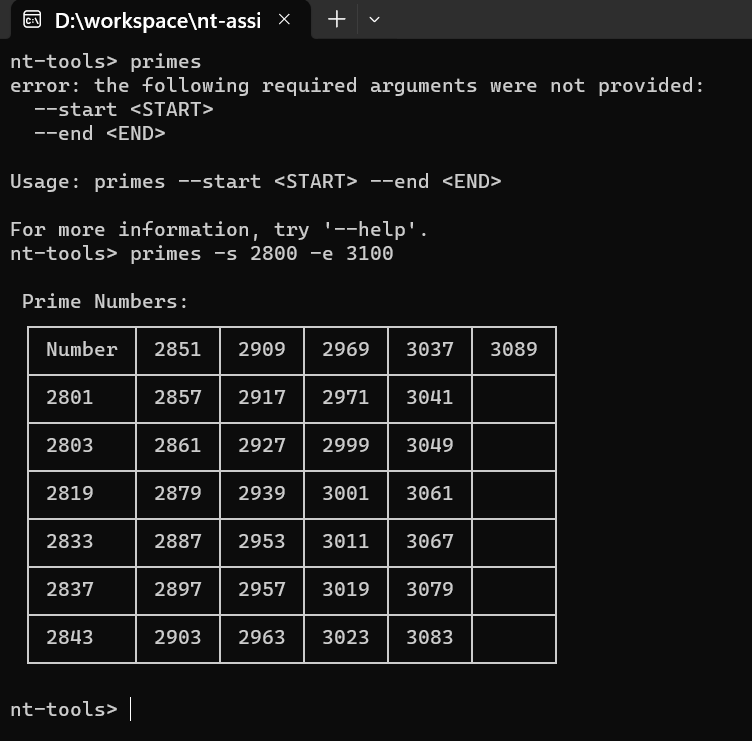
\includegraphics[scale=0.4]{list_primes.png}
            \caption{List of prime numbers in a range}
        \end{figure}

        \item composites
        \begin{lstlisting}[style=DOS]

        composites --start 2800 --end 3100
        \end{lstlisting}

        The below screenshot shows a sample output:
        \begin{figure}[H]
            \centering
            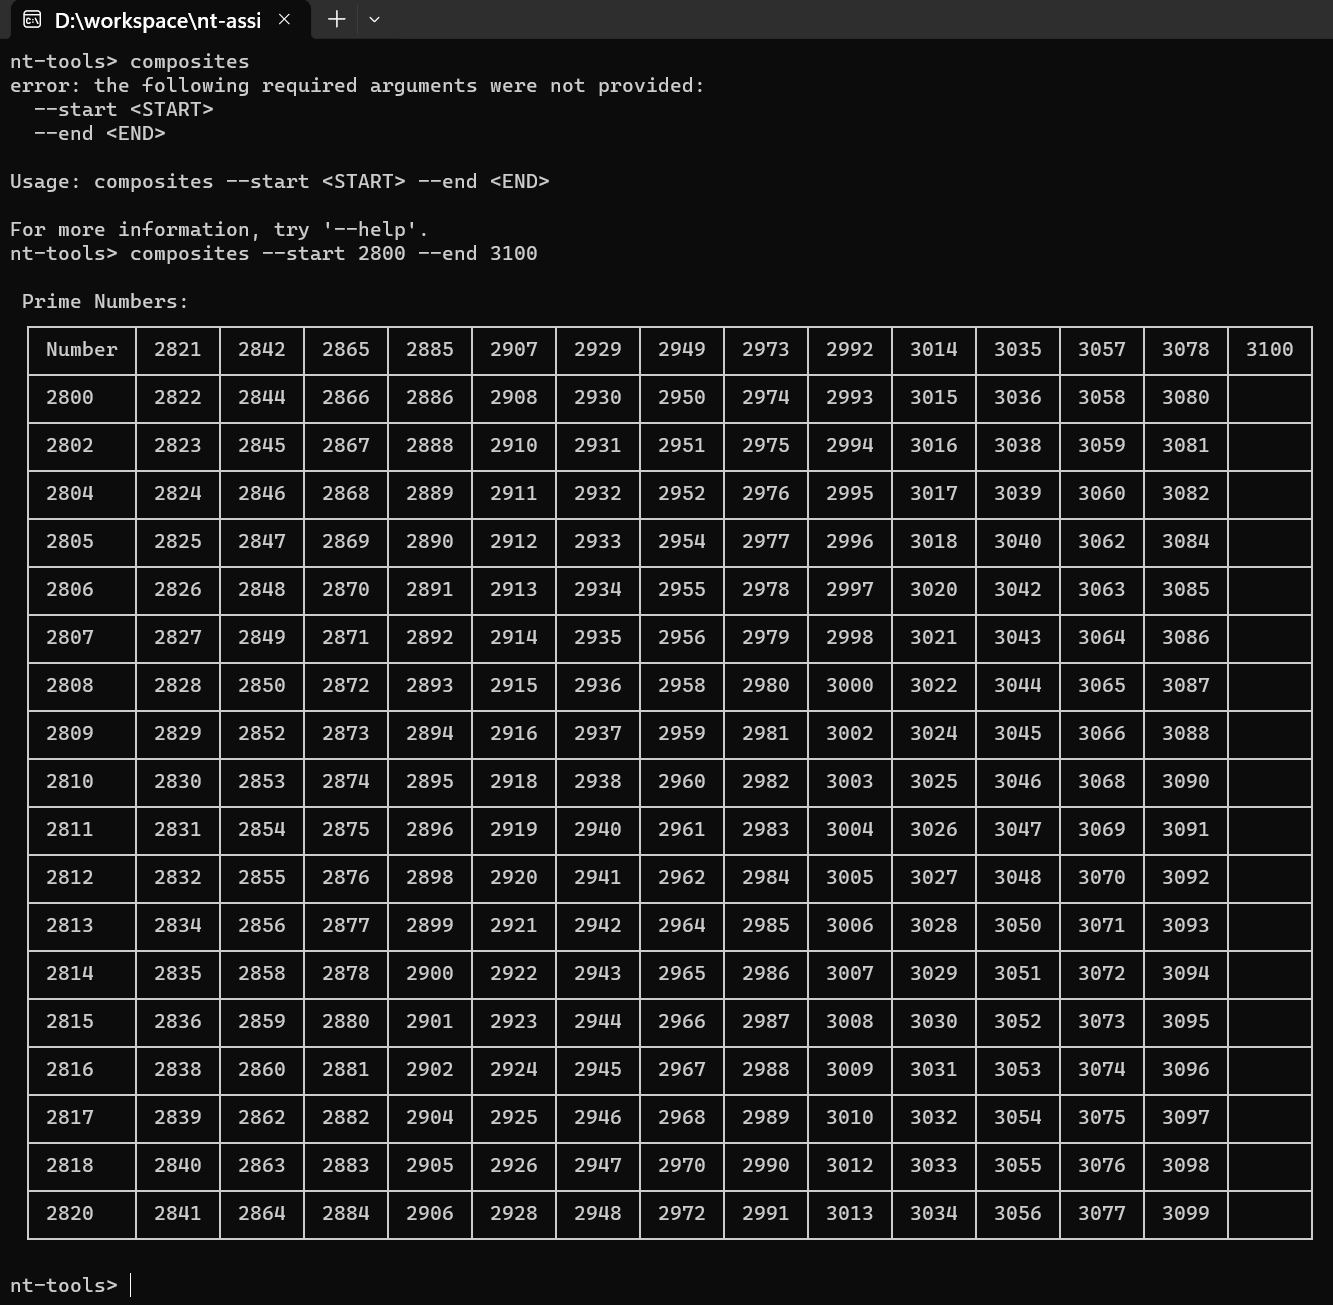
\includegraphics[scale=0.4]{list_composites.png}
            \caption{List of composite numbers in a range}
        \end{figure}

        \item composites-pq
        \begin{lstlisting}[style=DOS]

        composites-pq --start 2800 --end 3100
        \end{lstlisting}

        The below screenshot shows a sample output:
        \begin{figure}[H]
            \centering
            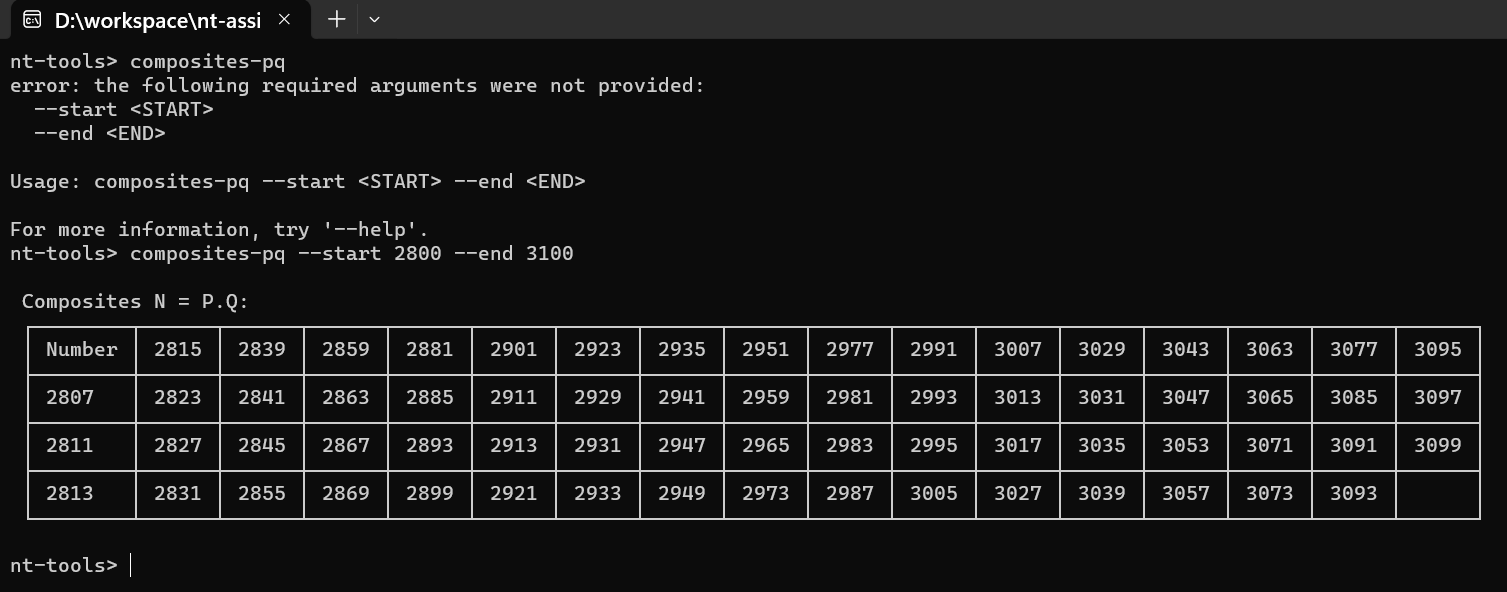
\includegraphics[scale=0.4]{composites-pq_list.png}
            \caption{List of composite numbers of the form N = P.Q in a range}
        \end{figure}

        \item nums-with-primitive-roots
        \begin{lstlisting}[style=DOS]

        nums-with-primitive-roots --start 600 --end 750
        \end{lstlisting}

        The below screenshot shows a sample output:
        \begin{figure}[H]
            \centering
            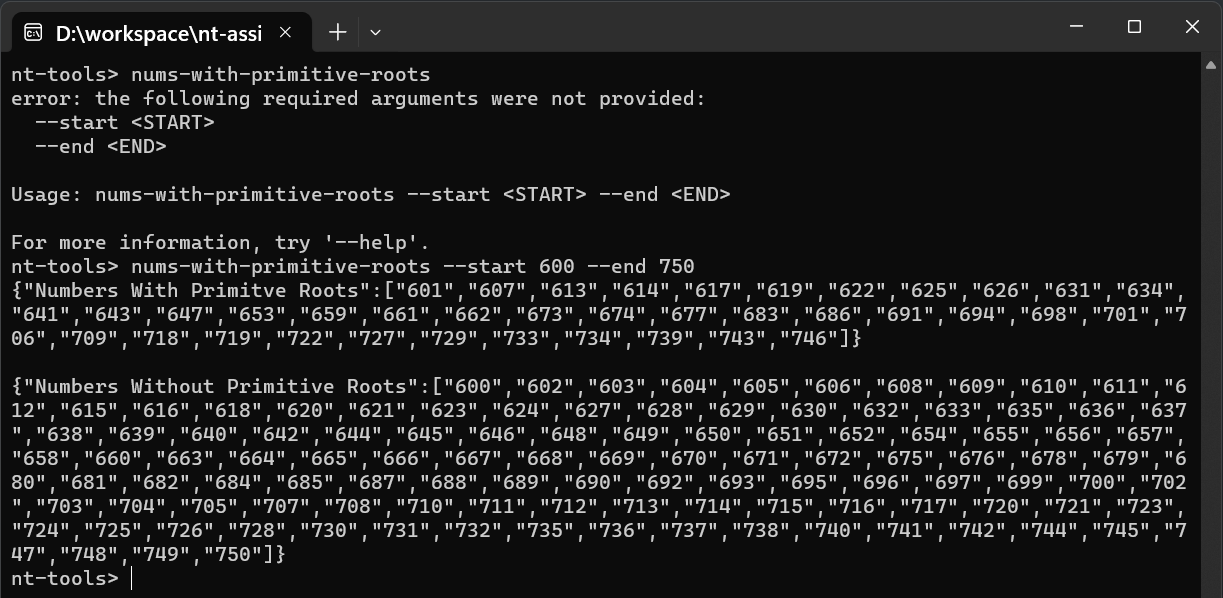
\includegraphics[scale=0.4]{nums-with-primitive-roots_list.png}
            \caption{List of numbers with primitive roots in a range}
        \end{figure}

        \item carmichael-nums
        \begin{lstlisting}[style=DOS]
        # Carmichael Numbers using FLT
        1. carmichael-nums --method fermat --start 2800 --end 3100

        # Carmichael Numbers using Korselt criteria
        2. carmichael-nums --method korselt --start 2800 --end 3100
        \end{lstlisting}

        The below screenshot shows a sample output:
        \begin{figure}[H]
            \centering
            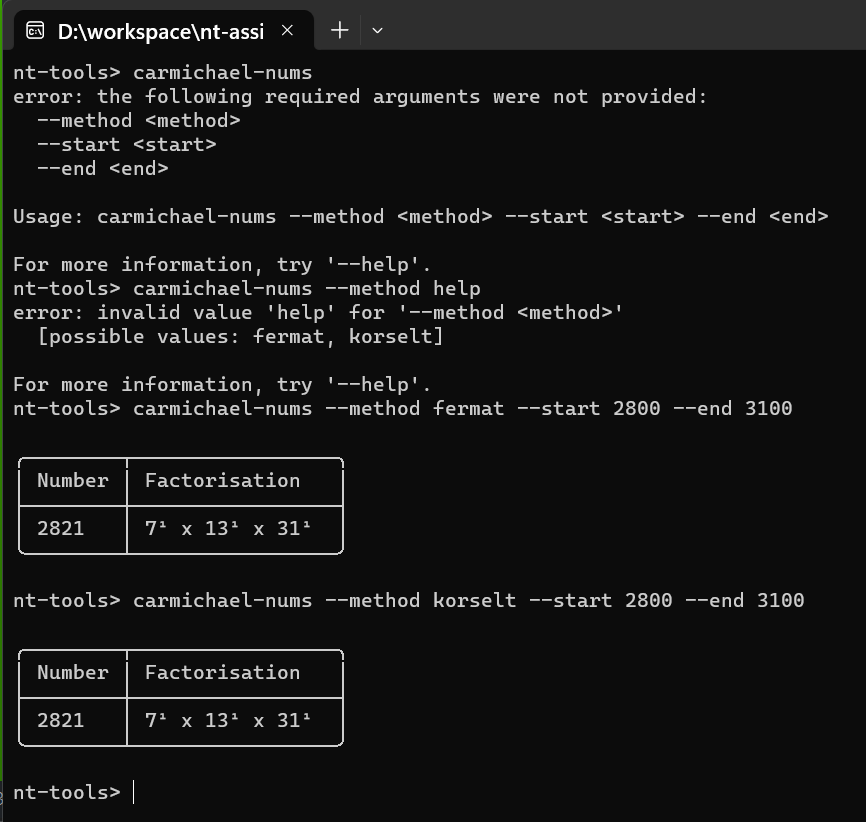
\includegraphics[scale=0.4]{carmichael-nums_list.png}
            \caption{Carmichael Numbers in a range}
        \end{figure}

        \item ifactors
        \begin{lstlisting}[style=DOS]
        # Integer Factorisation of a single number using trial and error
        1. ifactors --num1 2452

        # Integer factorisation of a range of numbers
        2. ifactors --num1 2800 --num2 2850
        \end{lstlisting}

        The below screenshot shows a sample output:
        \begin{figure}[H]
            \centering
            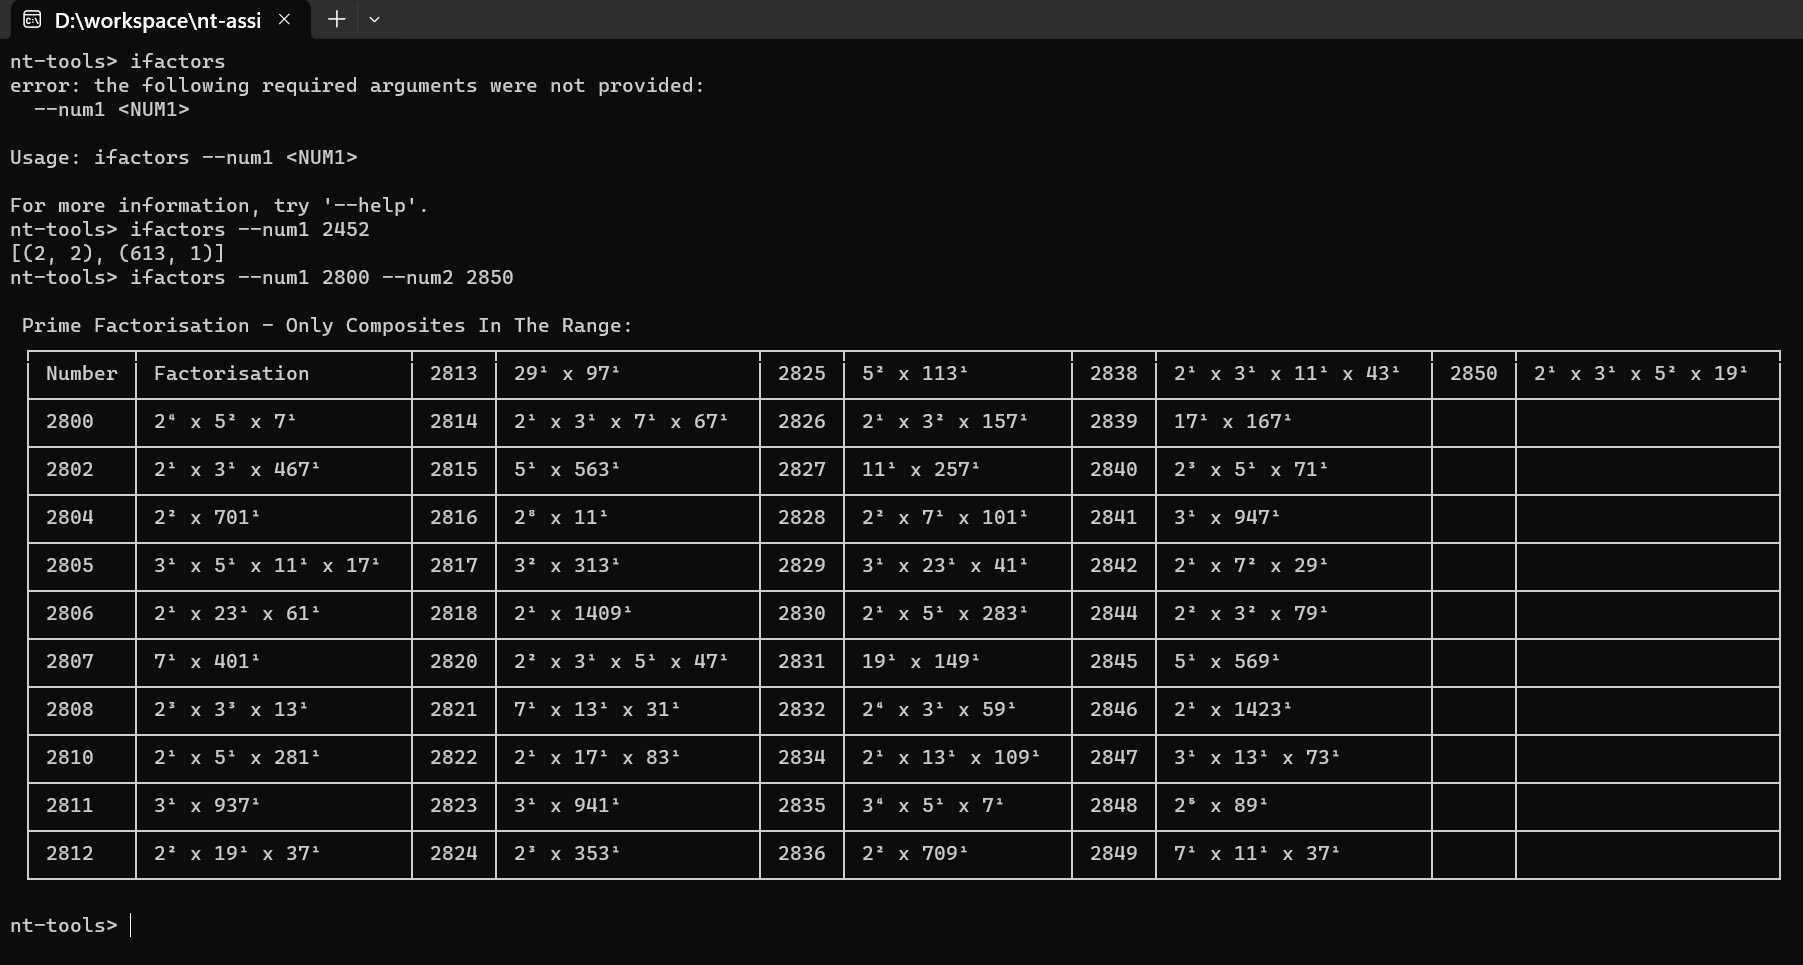
\includegraphics[scale=0.35]{ifactors.png}
            \caption{Integer Factorisation}
        \end{figure}

        \item primality
        \begin{lstlisting}[style=DOS]

        # Primality check using gcd test
        primality --method gcd --num 71

        # Primality check using trial division
        primality --method trial-division --num 71

        # Primality check using Miller Rabin
        primality --method miller-rabin --num 71

        # Primality check using AKS Algm
        primality --method aks --num 71

        # Primality check using FLT - Not Implemented
        primality --method fermat --num 71
        \end{lstlisting}

        The below screenshot shows a sample output:
        \begin{figure}[H]
            \centering
            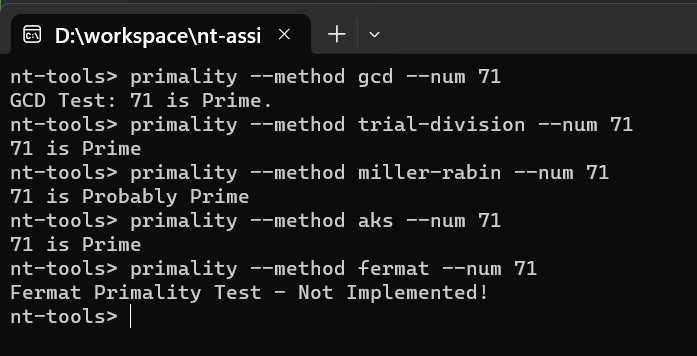
\includegraphics[scale=0.5]{primality.png}
            \caption{List of prime numbers in a range}
        \end{figure}

        \item miller-rabin-liars
        \begin{lstlisting}[style=DOS]

        miller-rabin-liars --num 2869
        \end{lstlisting}

        The below screenshot shows a sample output:
        \begin{figure}[H]
            \centering
            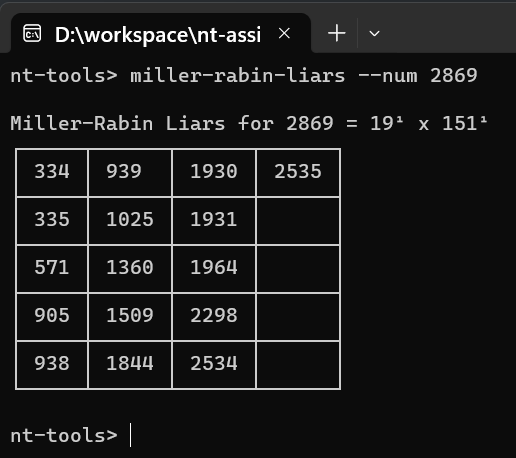
\includegraphics[scale=0.4]{miller-rabin-liars.png}
            \caption{Find the Miller-Rabin Liars of a number}
        \end{figure}

        \item gcd
        \begin{lstlisting}[style=DOS]

        gcd --num1 2000 --num2 200
        \end{lstlisting}

        The below screenshot shows a sample output:
        \begin{figure}[H]
            \centering
            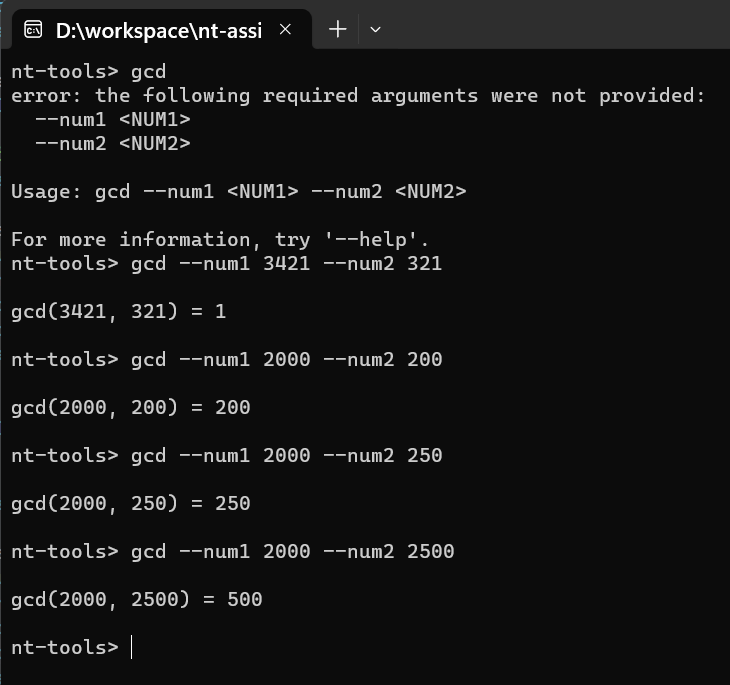
\includegraphics[scale=0.4]{gcd.png}
            \caption{GCD of two numbers}
        \end{figure}

        \item quadratic-sieve
        \begin{lstlisting}[style=DOS]

        quadratic-sieve --num 391
        \end{lstlisting}

        The below screenshot shows a sample output:
        \begin{figure}[H]
            \centering
            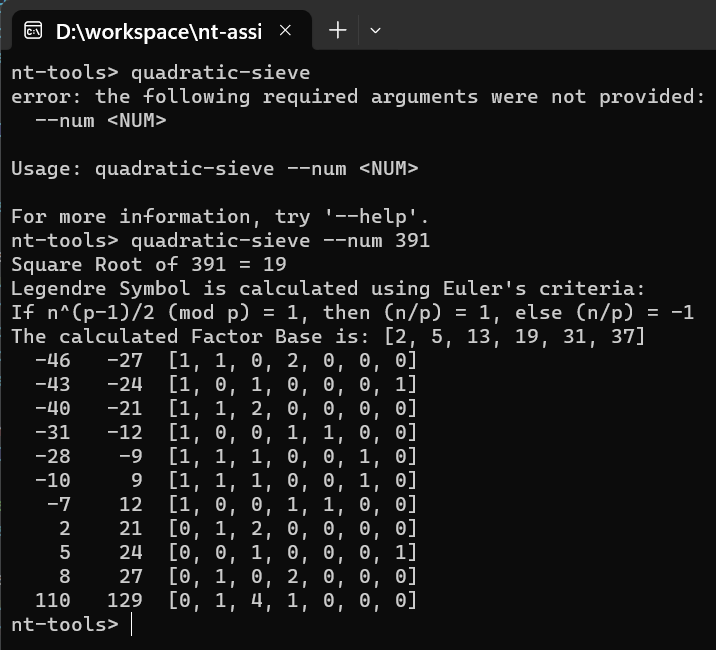
\includegraphics[scale=0.4]{quadratic-sieve.png}
            \caption{Quadratic Sieve Evaluation Matrix}
        \end{figure}

        \item pollards-p-minus-1
        \begin{lstlisting}[style=DOS]

        pollards-p-minus-1 --num 78719 --base 13
        \end{lstlisting}

        The below screenshot shows a sample output:
        \begin{figure}[H]
            \centering
            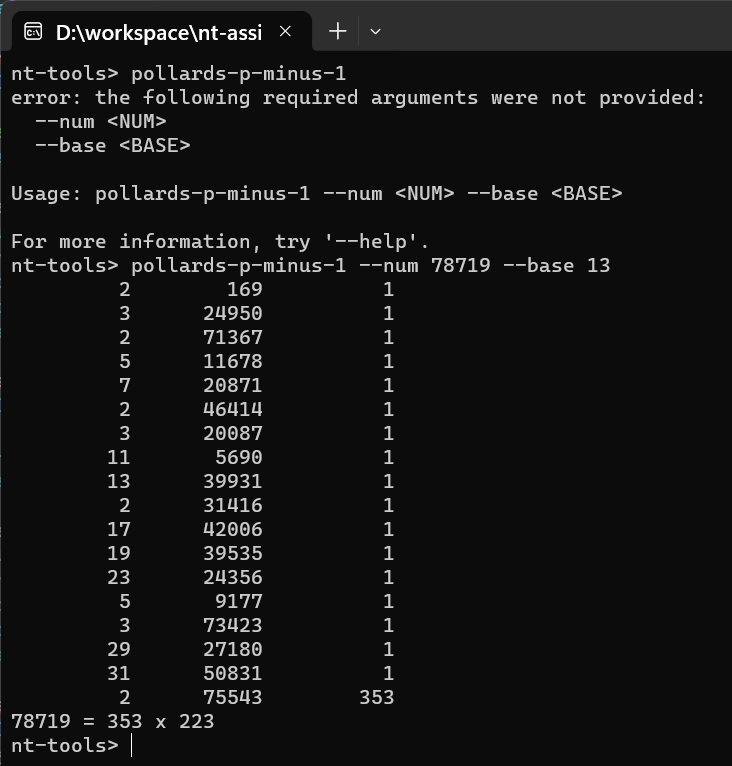
\includegraphics[scale=0.4]{pollards-p-minus-one.png}
            \caption{Pollard's P-1 Factorisation}
        \end{figure}

        \item pollards-rho
        \begin{lstlisting}[style=DOS]

        pollards-rho --primitive-root 21 -b 47 -m 71
        \end{lstlisting}

        The below screenshot shows a sample output:
        \begin{figure}[H]
            \centering
            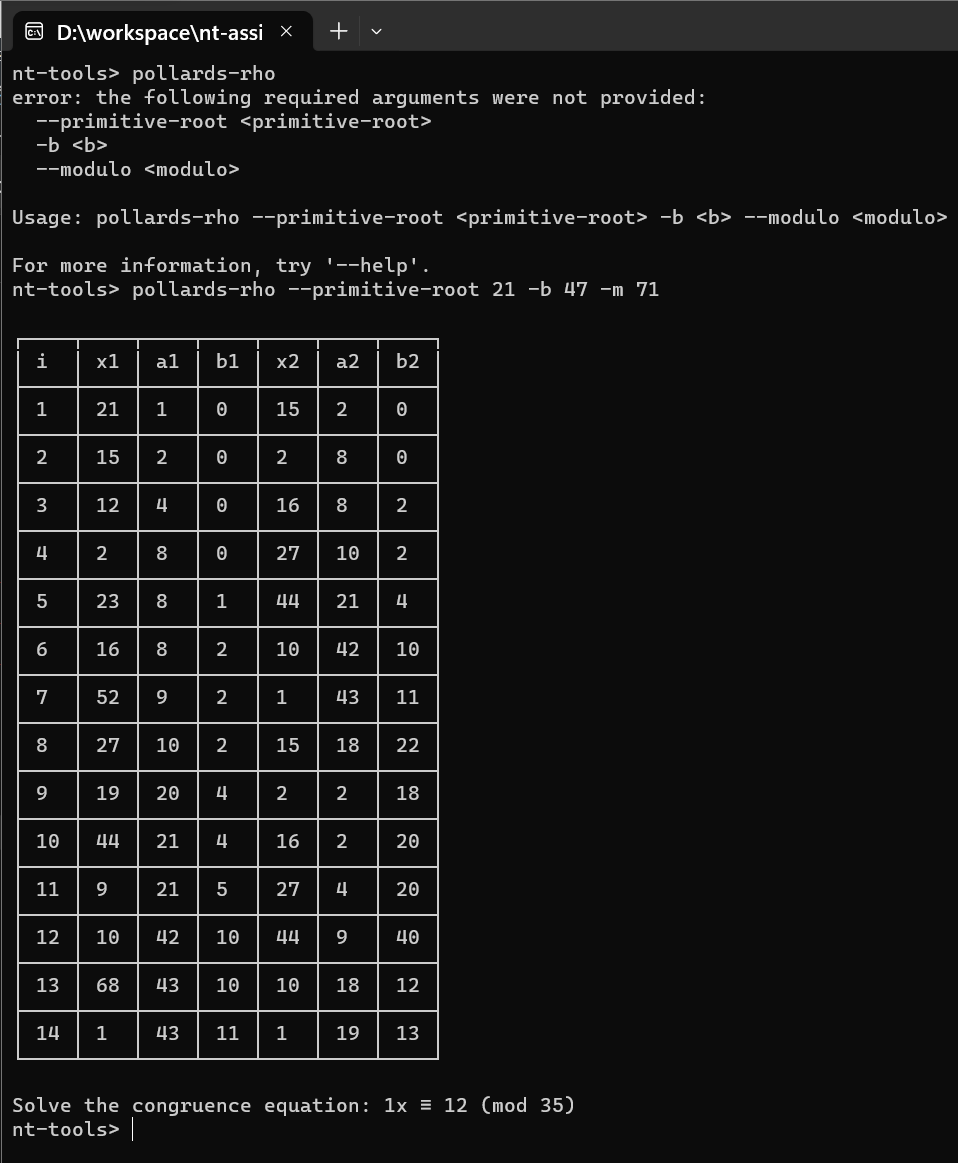
\includegraphics[scale=0.5]{pollards-rho.png}
            \caption{Discrete Logarithm - Pollard's Rho}
        \end{figure}

        \item modular-pow
        \begin{lstlisting}[style=DOS]

        modular-pow -b 26 -e 32 -m 53
        \end{lstlisting}

        The below screenshot shows a sample output:
        \begin{figure}[H]
            \centering
            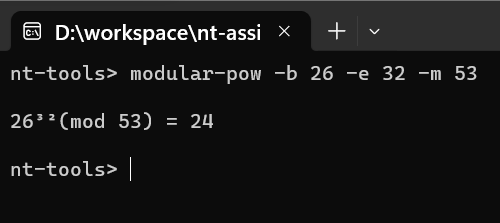
\includegraphics[scale=0.5]{mod-pow.png}
            \caption{Modular Exponentiation}
        \end{figure}

        \item aks-findr
        \begin{lstlisting}[style=DOS]

        aks-findr --num 71
        \end{lstlisting}

        The below screenshot shows a sample output:
        \begin{figure}[H]
            \centering
            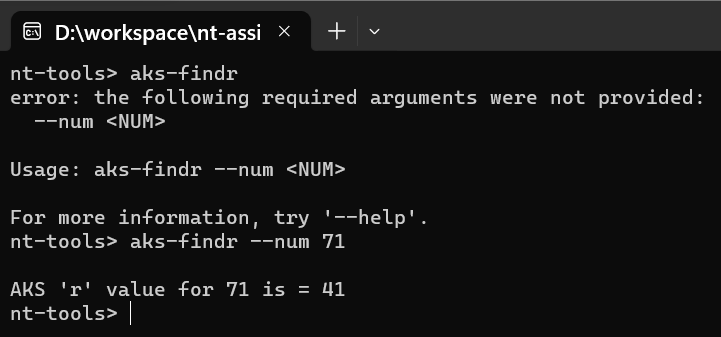
\includegraphics[scale=0.4]{aks-findr.png}
            \caption{'r' value of AKS Algm}
        \end{figure}

        \item list-primitive-roots
        \begin{lstlisting}[style=DOS]

        list-primitive-roots --num 17
        \end{lstlisting}

        The below screenshot shows a sample output:
        \begin{figure}[H]
            \centering
            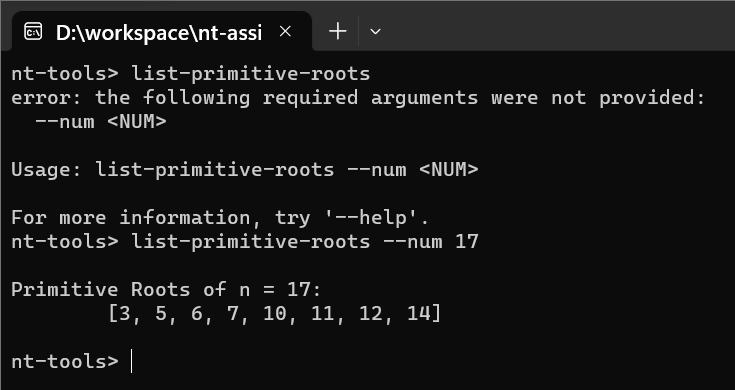
\includegraphics[scale=0.4]{list_primitive-roots.png}
            \caption{List Primitive Roots of a number}
        \end{figure}

        \item ass2q2b
        \begin{lstlisting}[style=DOS]

        ass2q2b --start 50 --end 100
        \end{lstlisting}

        The below screenshot shows a sample output:
        \begin{figure}[H]
            \centering
            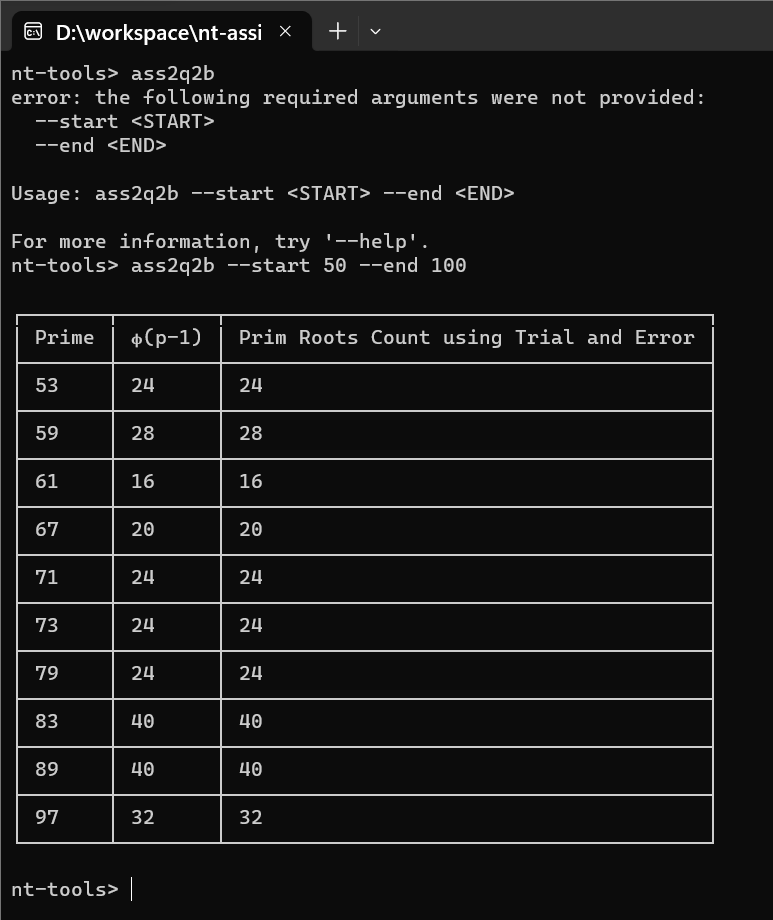
\includegraphics[scale=0.5]{primitive-roots-count.png}
            \caption{Assignment No. 2 Question 2(b) - Number of Primitive Roots}
        \end{figure}

        \item ass2q2c
        \begin{lstlisting}[style=DOS]

        ass2q2c --start 50 --end 100
        \end{lstlisting}

        The below screenshot shows a sample output:
        \begin{figure}[H]
            \centering
            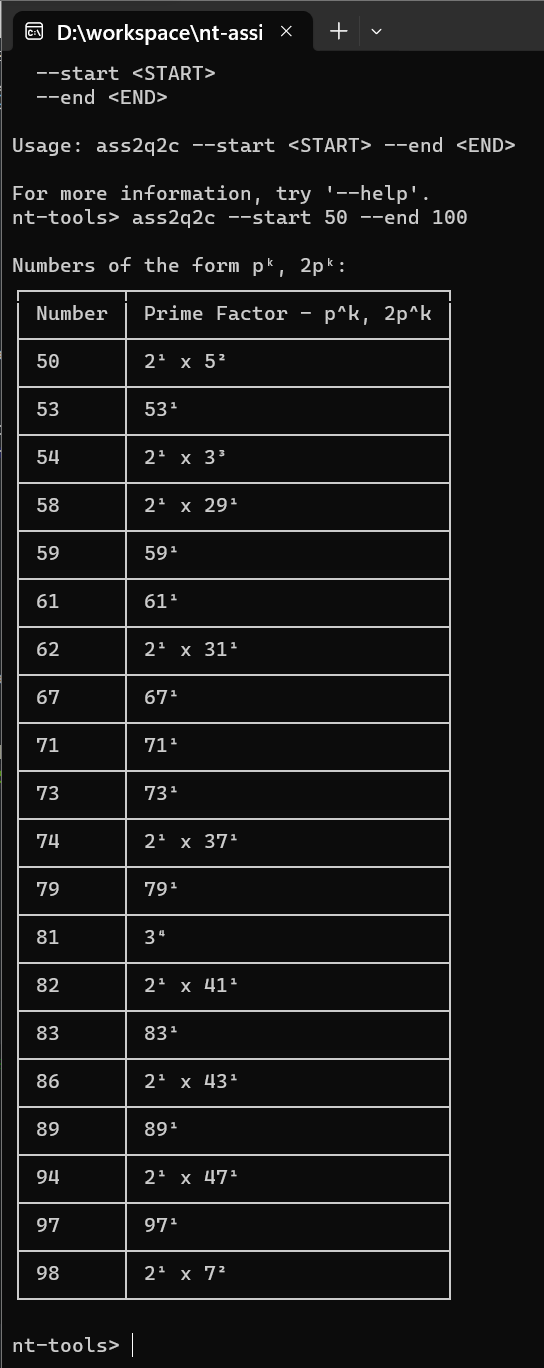
\includegraphics[scale=0.5]{p_k_2p_k.png}
            \caption{Number's of the form $p^k, 2p^k$}
        \end{figure}

        \item ass2q3d
        \begin{lstlisting}[style=DOS]

        ass2q3d --start 2800 --end 2850
        \end{lstlisting}

        The below screenshot shows a sample output:
        \begin{figure}[H]
            \centering
            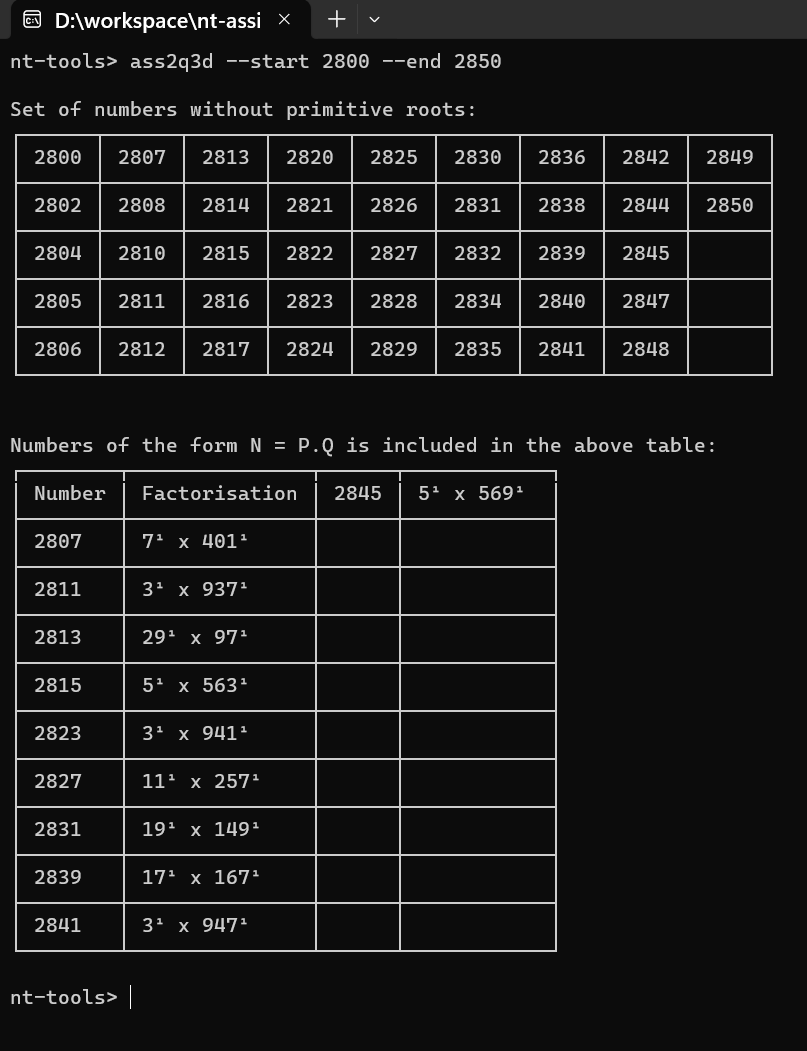
\includegraphics[scale=0.4]{ass2q3d.png}
            \caption{Primitive Roots \& Numbers of form N = P.Q}
        \end{figure}

        \item aks-failed-steps-for-n
        \begin{lstlisting}[style=DOS]

        aks-failed-steps-for-n --start 2800 --end 3100
        \end{lstlisting}

        The below screenshot shows a sample output:
        \begin{figure}[H]
            \centering
            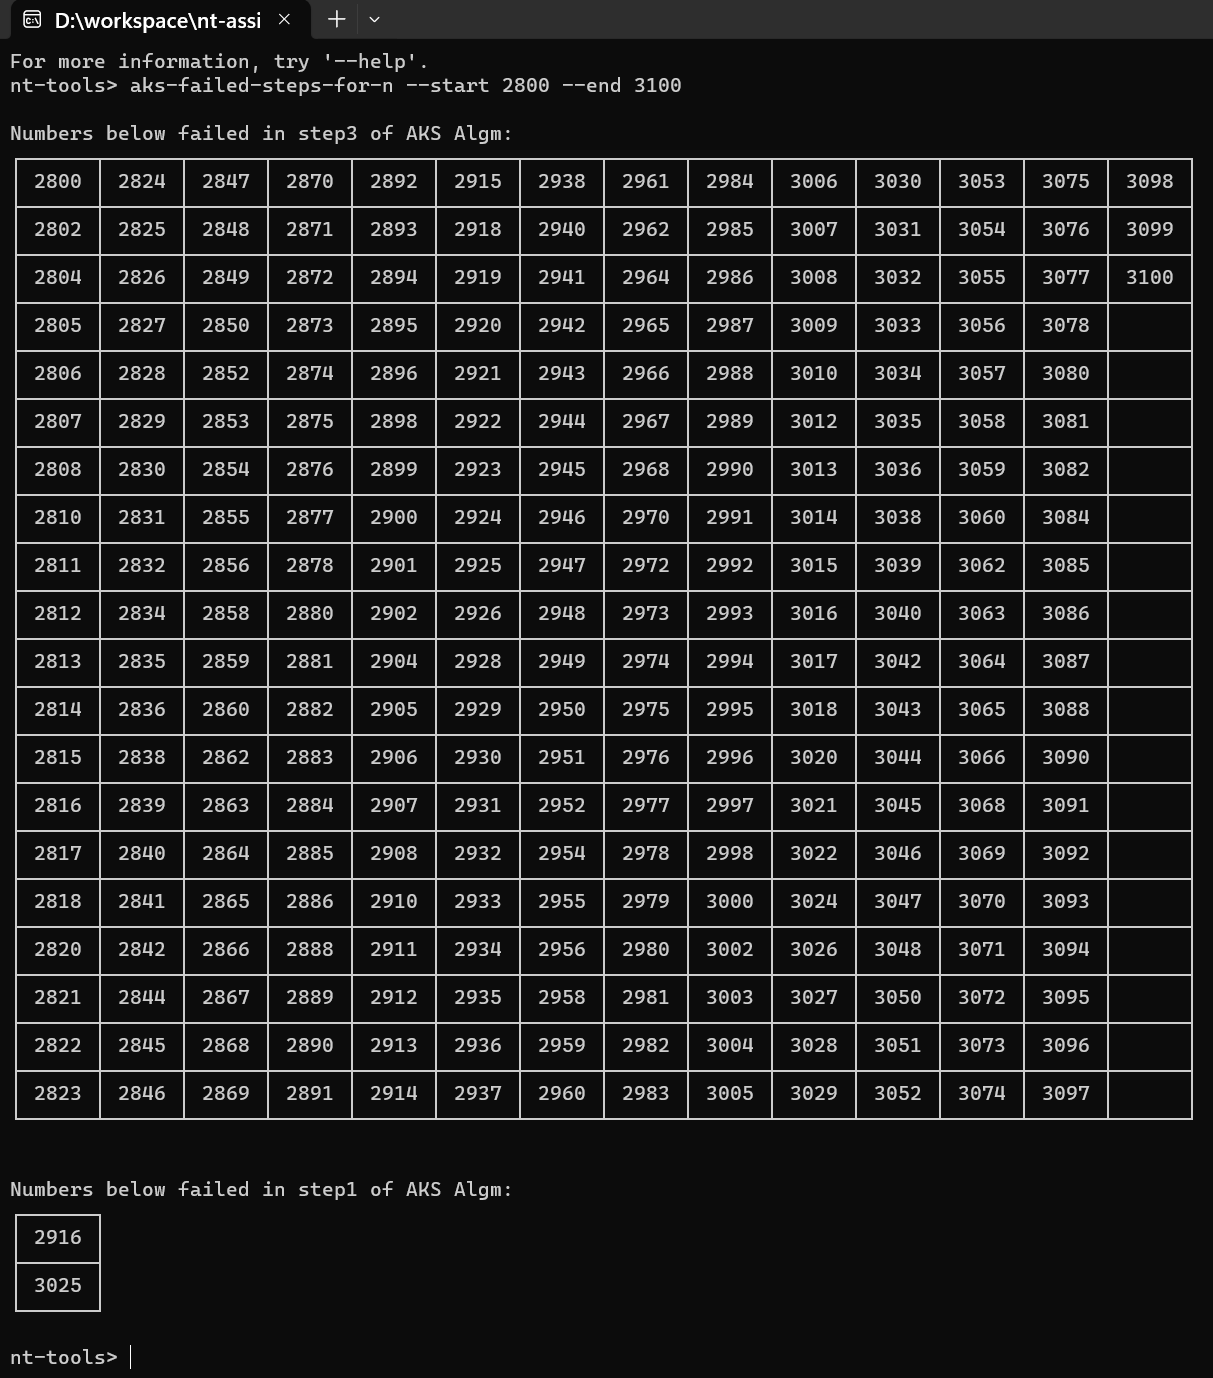
\includegraphics[scale=0.4]{aks-failure-steps.png}
            \caption{List of numbers failed the AKS at each of steps}
        \end{figure}

        \item clear or cls\\

        Clears the screen.
        \item quit or exit
    \end{enumerate}

\end{document}